
\chapter[Contribution to CO-Optimal Transport]{Contribution to CO-Optimal Transport}

\renewcommand{\contentsname}{Contents}
\localtableofcontents*
\chaptermark{\textbf{Contribution to CO-Optimal Transport}}

\hfill \break
This chapter presents two contributions to the CO-Optimal Transport (COOT).
The first one is summarized in \citep{Tran21},
which studies a relaxation of COOT via multi-marginal OT (MMOT).
It unifies several popular OT methods under its umbrella by promoting structural information
on the coupling. We show that incorporating such information into MMOT results in an
instance of a difference of convex (DC) programming problem allowing us to solve it numerically.
Despite high computational cost, the solutions provided by DC optimization are usually
as qualitative as those obtained using currently employed optimization schemes.

The second contribution is on the continuous COOT and its entropic approximation.
We consider a generalization of measure network called \textit{measure hypernetwork}
and show that continuous COOT can be used to compare such objects.
We then study the convergence behavior of the entropic approximation of COOT in the finite-dimensional
setting. Furthermore, under the GW framework, we can quantify the approximation error of
entropic COOT and easily extend this analysis to the GW distance.

\textbf{Important note:} \textit{This second contribution is based on my unpublished working paper
on continuous COOT in November 2021 and bears similarity with two concurrent works.
The first one is the hypergraph COOT \citep{Chowdhury21b} published in December 2021.
Their work and ours are based on the same mathematical framework of \citep{Chowdhury19},
which results in the same metric property. Apart from that, they pursue different research objectives,
where COOT is used to explore the categorical properties of the space of measure hypernetworks.
By contrast, we consider continuous COOT as the first step towards the analysis of
entropic approximation, unbalanced extension and sample complexity.}

\textit{Our study on the entropic COOT also shares some resemblance to the approximation error of
entropic GW in the paper of \citep{Zhang23} published in December 2022.
Their analysis and ours use the block approximation technique \citep{Carlier17}
to show the convergence of the minimum and minimizer, and to quantify the approximation error.
In particular, our result can be immediately extended to the GW setting. However,
we consider different assumptions on the mm-spaces,
which imply different upper bound of the approximation error.}

\raggedbottom

%%%%%%%%%%%%%%%%%%%%%%%%%%%%%%%%%%%%%%%%%%%%%%%%%%
\section{Background on discrete CO-Optimal Transport}

In many practical applications, the tabular data are usually expressed as a matrix whose rows
represent samples and columns represent features.
In general, the usual OT-based divergences, notably the Wasserstein and GW distances, mostly make
use of the pairwise distances, either within or across domains, to construct the cost matrix
or tensor. This approach has two consequences. First, only sample correspondences are of interest,
By contrast, one completely discards the feature alignments, which can be also interpretable,
for example, in single-cell multi-omics tasks \citep{Demetci20b}.
\footnote{In case of Wasserstein distance, there is no interest of feature correspondences
because intuitively, they are equivalent to the identity matrix. However,
it is no longer clear how to identify the such matching in the GW setting.}.
Second, the distance averages out the features, thus incurs information loss.
This can be problematic in the high-dimensional setting,
where the Euclidean distance is usually not a good metric
(see for example, \citep{Aggarwal01}, or Theorem 3.1.1 and Remark 3.1.2 in \citep{Vershynin18})
\footnote{For more informative discussion,
see \url{https://stats.stackexchange.com/questions/99171/why-is-euclidean-distance-not-a-good-metric-in-high-dimensions}.}.

One way to overcome these limitations is to use the \textit{Co-Optimal Transport} (COOT)
\citep{Redko20}, which learns simultaneously the sample and feature alignments.
In what follows, we denote by $\Delta_{n}= \{p \in \bbR_{> 0}^n: \sum_{i=1}^{n} p_{i}=1\}$
the simplex histogram with $n$ bins. We call $\cX = (X, \mu_1^X, \mu_2^X)$ a \textit{weighted matrix}
defined by a triplet comprised of a matrix $X \in \bbR^{n_x \times d_x}$
equipped with the histograms $\mu_1^X \in \Delta_{n_x}$ and $\mu_2^X \in \Delta_{d_x}$
on its rows and columns, respectively. For $p \geq 1$, we define the COOT between two
weighted matrices $\cX = (X, \mu_1^X, \mu_2^X)$ and $\cY = (Y, \mu_1^Y, \mu_2^Y)$ as
\begin{align}
  \label{eq:discrete_coot}
    \coot(\cX, \cY) :=
    \inf_{\substack{P \in U(\mu_1^X, \mu_1^Y) \\ Q \in U(\mu_2^X, \mu_2^Y)}}
    \sum_{i,j,k,l} (X_{ij} - Y_{kl})^p P_{ik} Q_{jl}.
\end{align}
By Proposition 1 in \citep{Redko20}, if the weights are uniforms,
then COOT defines a distance on the space of weighted matrices,
up to permutation of the matrix coordinates. We note that the formulation \eqref{eq:discrete_coot}
can be easily extended to the multi-coupling setting, for example, in \citep{Kerdoncuff22}.
% They show has shown strong performance of the proposed method in
% heterogeneous domain adaptation.

From the perspective of matrix-comparison, COOT provides a principled way
to compare any two arbitrary-size matrices. By contrast,
this is not the case for many other existing divergences,
whose applicability is summarized in \Cref{t:comparisons}.
\begin{table}[h]
	\centering
		\begin{tabular}{|l|l|l|}
    \hline
    \textbf{Divergences} & \textbf{Input matrices} & \textbf{Requirement on histograms} \\
    \hline
    Matrix norms & Same-size matrices & Not applicable \\
    \hline
    OT, UOT, SW & \makecell[l]{Matrices with the same \\ number of columns}
    & Only requires histogram on rows \\
    \hline
    GW, FGW, UGW, SGW & Square matrices & \makecell[l]{Histograms on rows and columns \\ must be the same} \\
    \hline
    COOT & Arbitrary-size matrices & \makecell[l]{Any histograms on rows and columns} \\
    \hline
		\end{tabular}
		\caption{Applicablility of some popular divergences. COOT is much more flexible than
    other OT-based divergences. UOT and UGW are the unbalaced OT and unbalaced GW divergence, respectively.
    FGW is the Fused GW divergence. SW and SGW denote the sliced Wasserstein \citep{Rabin12,Bonneel15}
    and sliced GW \citep{Vayer19a} distances.
    \label{t:comparisons}}
\end{table}

\paragraph{Co-Optimal Transport as lower bound of GW distance} \label{subsec:GWLB}
Under the framework of discrete GW, where the inputs are similarity matrices, for simplicity,
we write $\cX = (C^x, \mu_X)$, where $C^x$ is the similarity matrix and
$\mu_X$ is the sample histogram. Now, the GW distance can be reformulated as
\begin{align}
  \label{eq:discrete_gw_coot}
  \gw(\cX, \cY) =
  \inf_{\substack{P, Q \in U(\mu_X, \mu_Y) \\ P=Q}}
  \sum_{i,j,k,l} (C^x_{ij} - C^y_{kl})^p P_{ik} Q_{jl},
\end{align}
meaning that we optimize with respect to two independent couplings
under the additional constraint that they must be equal. If it is relaxed, then
one recovers the COOT distance between $\cX$ and $\cY$. We also stress that COOT should not
be confused with the third lower bound of the GW distance \citep{Memoli07,Memoli11} defined as
\begin{equation}
  \text{TLB}(\cX, \cY) :=
  \inf_{Q \in U(\mu_X, \mu_Y)}
  \Big( \inf_{P \in U(\mu_X, \mu_Y)} \sum_{i,j,k,l} (C^x_{ij} - C^y_{kl})^p P_{ik} \Big) Q_{jl}.
\end{equation}
In particular, we have $\gw(\cX, \cY) \geq \coot(\cX, \cY) \geq \text{TLB}(\cX, \cY)$.

% The equivalence between BAP and QAP has already been studied in \citep{Konno76}.
If the inputs are the Euclidean, or squared Euclidean distances, then equality holds between
COOT and GW distances \citep{Sejourne20,Redko20}. These results are based on the prior works
of \citep{Konno76,Maron18} and summarized in the folllowing proposition.
\begin{definition}
  A square matrix $A \in \bbR^{n \times n}$ is conditionally negative semi-definite (CND)
  if it is symmetric and for any $c \in \bbR^n$ such that $\sum_i c_i = 0$, we have
  $c^T A c \leq 0$.
\end{definition}
%%%%%%%%%%%%%%%%%%%%%%%%%%%%%%%%%%%%%%%%%%%%%%%%%%%%%%%%
\begin{proposition}
  \label{prop:coot_gw_equiv}
  For $p=2$, suppose that $C^x$ and $C^y$ are of the forms:
  $C^x_{ij} = f_i + f_j + A_{ij}$ and $C^y_{kl} = g_k + g_l + B_{kl}$,
  where $f, g$ are vectors in $\bbR^m, \bbR^n$, respectively,
  and the matrices $A, B$ are CND. Then $\gw(\cX, \cY) = \coot(\cX, \cY)$.
  Furthermore, if $(P_1^*, P_2^*)$ is a solution of the COOT problem, then $P_1^*$ and $P_2^*$
  are two solutions of the GW problem. In particular,
  if the semi-definiteness is replaced by the definiteness, then $P_1^* = P_2^*$.
\end{proposition}
Roughly speaking, if the similarity matrices is "approximately" CND,
then one can safely remove the equality constraint without changing the minimum.
Thus, \Cref{prop:coot_gw_equiv} justifies the rationale behind
the alternative minimization procedure for GW distance presented in \Cref{subsec:gw_approx}.
This scheme is easily adapted to the entropic fused GW problem, by observing that,
for any reference histogram $\mu \in \bbR_{> 0}^{m \times n}$, we have
\begin{equation}
  \begin{split}
    &\inf_{\substack{P \in U(\mu_X, \mu_Y)}}
  \sum_{i,j,k,l} (C^x_{ij} - C^y_{kl})^p P_{ik} P_{jl}
  + \alpha \langle D, P \rangle + \varepsilon \; \kl(P | \mu) \\
  &= \inf_{\substack{P \in U(\mu_X, \mu_Y) \\ Q \in U(\mu_X, \mu_Y) \\ P = Q }}
  \sum_{i,j,k,l} (C^x_{ij} - C^y_{kl})^p P_{ik} Q_{jl}
  + \frac{\alpha}{2} \langle D, P \rangle + \frac{\alpha}{2} \langle D, Q \rangle
  + \frac{\varepsilon}{2} \kl(P | \mu) + \frac{\varepsilon}{2} \kl(Q | \mu).
  \end{split}
\end{equation}
Again, under exactly the same conditions on the similarity matrices in \Cref{prop:coot_gw_equiv},
one can safely drop the equality constraint during the optimization.

%%%%%%%%%%%%%%%%%%%%%%%%%%%%%%%%%%%%%%
\section{Continuous Co-Optimal Transport}
%%%%%%%%%%%%%%%%%%%%%%%%%%%%%%%%%%%%%%

In this section, we present our unpublished work on the continuous COOT and its entropic approximation.
We will mostly follow the terminology and concepts proposed in the published work of \citep{Chowdhury21b}.

\subsection{Formulation and preliminary results}

As already seen in discrete GW problem \eqref{eq:discrete_gw_coot},
by rewriting a measure network $\cX = (X, c_X, \mu_X)$ as
$\widetilde{\cX} = \big((X_1, \mu_1^X), (X_2, \mu_2^X), c_X \big)$, with
$X_1 = X_2 = X$ and $\mu_1^X = \mu^X_2 = \mu_X$, one can reformulate the GW problem as
\begin{equation}
  \begin{split}
    \inf_{\pi_1, \pi_2}
    &\int_{X_1 \times Y_1} \int_{X_2 \times Y_2}
    \big\vert c_X(x_1, x_2) - c_Y(y_1, y_2) \big\vert^p \; d\pi_1(x_1, y_1) \; d\pi_2(x_2, y_2). \\
    \text{ subject to: } &\pi_k \in U(\mu_k^X, \mu_k^Y), \forall k = 1,2, \\
    &\pi_1 = \pi_2.
  \end{split}
\end{equation}
When the equality constraint on the two couplings is relaxed,
we can allow that either $X_1 \neq X_2$ or $Y_1 \neq Y_2$.
The interest of such situation can be found, for example, in heterogenous domain adaptation,
where $X_1$ and $Y_1$ represent the "sample" spaces in the source and target domains, respectively,
and $X_2$ and $Y_2$ represent the "feature" spaces in the source and target domains, respectively.
As a result, the corresponding "sample" and "feature" couplings are also different in their natures.

% Before defining the continuous extension of COOT, we need to specify the
% To this extent, we need to extend the prior work of \citep{Chowdhury19} on measure network.

\begin{definition}[Measure hypernetwork \citep{Chowdhury21b}]
Suppose $(X_1, \mu_1^X)$ and $(X_2, \mu_2^X)$ are two Polish measure spaces,
and $c_X$ is a bounded measurable function on $X_1 \times X_2$.
We call the triplet $\cX = \big((X_1, \mu_1^X), (X_2, \mu_2^X), c_X \big)$
a \textbf{measure hypernetwork}. We also say $c_X$ is the \textbf{interaction}
between $X_1$ and $X_2$.
\end{definition}
Without risk of confusion, when $X_1 = X_2 = X$ and $\mu_1^X = \mu_2^X = \mu_X$,
we use interchangeably "measure hypernetwork" and "measure network" in
the context of GW \citep{Chowdhury19}.
When $X_1$ and $X_2$ are finite spaces (so $\mu_1^X$ and $\mu_2^X$ are histograms),
we call $\cX$ a finite measure hypernetwork. For convenience, we also refer the index $1$ as "sample"
and $2$ as "feature", for example, $X_1$ is the sample space, $\pi_2$ is the feature coupling.
\begin{definition}[COOT distance between measure hypernetworks \citep{Chowdhury21b}]
  \label{def:cont_coot}
  For $p \geq 1$, the COOT distance between two measure hypernetworks $\cX$ and $\cY$ is defined as
  \begin{align} \label{eq:cont_coot}
    \coot(\cX, \cY) =
    \inf_{\substack{\pi_1 \in U(\mu^X_1, \mu^Y_1) \\
    \pi_2 \in U(\mu^X_2, \mu^Y_2)}} \iint
    \big\vert c_X(x_1, x_2) - c_Y(y_1, y_2) \big\vert^p \; d\pi_1(x_1, y_1) \; d\pi_2(x_2, y_2).
  \end{align}
\end{definition}
It is not difficult to see that \Cref{def:cont_coot} generalizes the discrete COOT \citep{Redko20}.
In practice, the input data is usually expressed as matrix,
whose rows represent samples and columns represent features.
In this case, the interaction value is precisely the coordinate of the data matrix.
Meanwhile, the sample and feature spaces are unknown and have little interest and importance.

% \begin{figure}[ht]
%   \centering
%   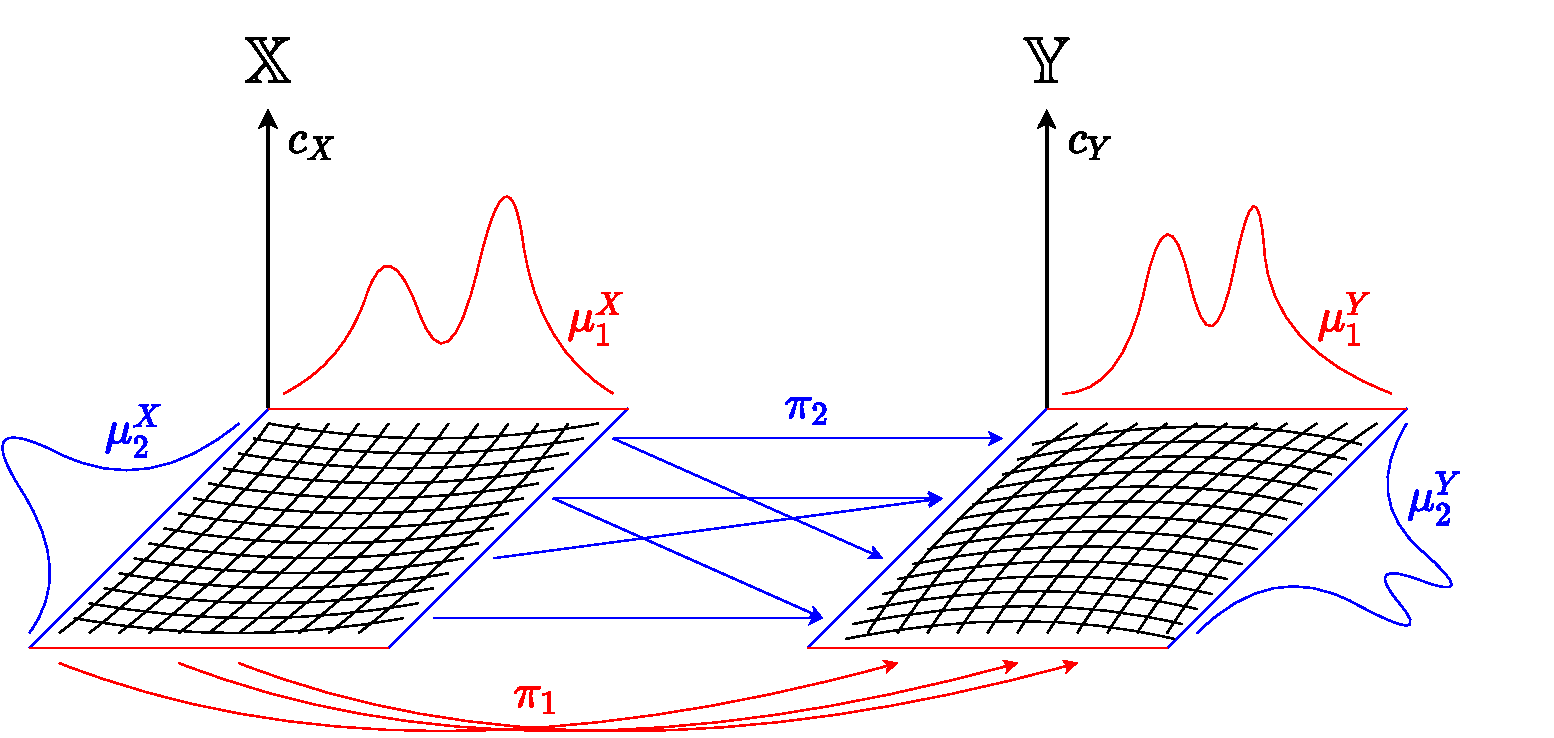
\includegraphics[width=0.9\textwidth, keepaspectratio]{./Chapitre2/fig/coot_diagram.pdf}
%   \caption{Scatter plots of MMOT-DC-v1 versus other solvers. In all three plots, the points tend to concentrate around the line $y=x$,
%   which indicates the comparable performance of MMOT-DC-v1. On the other hand, the top-right plot shows the clear superiority of EGW-PGD.}
%   \label{fig:continuous_coot}
% \end{figure}
First, we can show that the COOT problem \eqref{eq:cont_coot} is well defined.
\begin{proposition}[Lemma 35 in \citep{Chowdhury21b}]
  \label{prop:exist_coot}
  The COOT problem always admits a minimizer.
\end{proposition}
We provide the proof in Appendix \ref{annex:cont_coot}.
While the proofs of our result and of Lemma 35 in \citep{Chowdhury21b} use the same proof technique of
Theorem 2.2 in \citep{Chowdhury19}, ours is slightly different. More precisely,
we exploit a different reformulation of COOT, where it can be rewritten as a multi-marginal OT problem
with additional factorization constraint on the coupling. Later, we will see that,
this observation also allows to establish the convergence result of entropic COOT.

%%%%%%%%%%%%%%%%%%%%%%%%%%%%%%%%%%%%%%%%%%
\subsection{Metric properties}

The framework on the GW isomorphism presented in \Cref{subsec:prop_gw}
can be extended immediately to the COOT setting. In particular, while our
presentation is different to that of \citep{Chowdhury21b}, we still come up with the
same metric properties.


%%%%%%%%%%%%%%%%%%%%%%%%%%%%%%%%%%%%%%%%%
\begin{definition}[Relaxed mass splitting]
  A measure hypernetwork $\cZ$ is a \textbf{relaxed mass splitting} (RMS) of a
  measure hypernetwork $\cX$ if there exist two measure-preserving maps
  $\varphi_k: Z_k \to X_k$, for $k=1,2$, such that the pullback equality
  $c_Z = (\varphi_1, \varphi_2)^*c_X$ holds $\mu^Z_1 \otimes \mu_2^Z$-almost everywhere
  in $Z_1 \times Z_2$. We denote $\ms(\cX)$ the set of all mass splittings
  of $\cX$. This pair of maps $(\varphi_1, \varphi_2)$ is also called
  \textbf{basic weak isomorphism} in \citep{Chowdhury21b}.
\end{definition}
We denote $\rms(\cX)$ the set of all relaxed mass splittings of $\cX$. Clearly,
$\cX \in \rms(\cX)$, so $\rms(\cX)$ is not empty.
In particular, for measure networks, if $\cZ \in \ms(\cX)$, then $\cZ \in \rms(\cX)$,
meaning that $\ms(\cX) \subset \rms(\cX)$. Now, we can define the isomorphism between
the measure hypernetworks as follows.
\begin{definition}[COOT-isomorphism] \label{coot_isomorphic}
  Two measure hypernetworks are
  \begin{enumerate}
    \item strongly isomorphic if there exist two \textbf{bijective}
    measure-preserving map from one hypernetwork to the other such that the pullback equality holds
    \textbf{everywhere}.
    \item semi-strongly isomorphic if one is the RMS of the other and vice versa.
    \item weakly isomorphic if they have a common RMS.
  \end{enumerate}
\end{definition}
This is an immediate relaxation of the GW isomorphism. In particular,
in case of measure networks, isomorphism in GW sense implies COOT isormorphism.
The following result summarizes the relations amongst the three types of COOT isomorphism.
%%%%%%%%%%%%%%%%%%%%%%%%%%%%%%%%%%%%%%%%%%%%%%%%
\begin{corollary} \label{prop:strong_weak_iso}
  Given two measure hypernetworks $\cX$ and $\cY$. Consider three statements
  \begin{enumerate}
    \item[(1)] $\cX$ and $\cY$ are strongly isomorphism.
    \item[(2)] $\cX$ and $\cY$ are semi-strongly isomorphism.
    \item[(3)] $\cX$ and $\cY$ are weakly isomorphism.
  \end{enumerate}
  Then, the following relations hold
  \begin{enumerate}
    \item $(1) \implies (2) \implies (3)$.
    \item If $\cX$ and $\cY$ are finite, then $(2) \implies (1)$.
    \item If $\cX$ and $\cY$ are finite such that $|X_k| = |Y_k|$
    and $\mu_k^X, \mu_k^Y$ are uniform distributions, for $k = 1,2$, then
    $(3) \implies (2)$. This means all three forms are equivalent.
  \end{enumerate}
\end{corollary}
%%%%%%%%%%%%%%%%%%%%%%%%%%%%%%%%%%%%%%%%%%%%%%%%
Now, we can characterize the weak isomorphism by
\begin{proposition} \label{prop:coot_iso}
  Two measure hypernetworks $\cX$ and $\cY$ are COOT-weakly isomorphic if and only if
  $\coot(\cX, \cY) = 0$.
\end{proposition}
%%%%%%%%%%%%%%%%%%%%%%%%%%%%%%%%%%%%%%%%%%%%%%%%
\begin{proposition}[Theorem 1 in \citep{Chowdhury21b}] \label{prop:metric_prop}
  $\coot^{1/p}$ defines a metric on the space of measure hypernetworks, up to COOT-weak isomorphism.
\end{proposition}
%%%%%%%%%%%%%%%%%%%%%%%%%%%%%%%%%%%%%%%%%
% \paragraph{Discussion on the setting of mm-space}
% While the measure network can fit in the COOT framework, this is usually not the case for
% the mm-space since the distance function is only measurable in Polish space,
% but not necessarily bounded. However, all previous results on the existence of minimizer and
% metric property remain unchanged if one replaces measure hypernetworks by mm-spaces,
% as long as COOT is finite. Moreover,
% \begin{corollary}
% For $p=2$, all forms of COOT isomorphisms are equivalent and
% they are also equivalent to the isomorphism in GW sense.
% \end{corollary}
% This indicates that, both GW distance and COOT can be used to compare isometric objects,
% namely those transformed by reflection, rotation or translation.

%%%%%%%%%%%%%%%%%%%%%%%%%%%%%%%%%%%%%%%%%%%%%%%%
\subsection{Entropic regularization and approximation error}
%%%%%%%%%%%%%%%%%%%%%%%%%%%%%%%%%%%%%%%%%%%%%%%%
Similar to the Wasserstein and GW distances, one can approximate the COOT with entropic regularization.
In this thesis, we are interested in the following formulation of entropic COOT:
for $\varepsilon > 0$,
\begin{align}
  \coot_{\varepsilon} (\cX, \cY) =
  \inf_{\substack{\pi_1 \in U(\mu^X_1, \mu^Y_1) \\
  \pi_2 \in U(\mu^X_2, \mu^Y_2)}} &\iint
  \big\vert c_X(x_1, x_2) - c_Y(y_1, y_2) \big\vert^p \; d\pi_1(x_1, y_1) \; d\pi_2(x_2, y_2) \\
  &+ \varepsilon \; \kl \big( \pi_1 \otimes \pi_2 \vert (\mu^X_1 \otimes \mu^Y_1) \otimes (\mu^X_2 \otimes \mu^Y_2) \big).
\end{align}
Note that, this structure of the KL divergence term is particularly handy to prove all results related to
the entropic COOT. It also bears similarity with the \textit{quadratic divergence}
\citep{Sejourne20} defined by $\kl^{\otimes 2}(\mu, \nu):= \kl(\mu \otimes \mu | \nu \otimes \nu)$,
which is used to define the unbalanced GW divergence. Note that, in the balanced setting,
the joint penalization in terms of KL divergence is in fact equivalent to the
independent KL-penalization. More precisely, given any $\pi_k \in U(\mu_k^X, \mu_k^Y)$,
for $k=1,2$, we have
\begin{equation}
  \kl \big( \pi_1 \otimes \pi_2 \vert (\mu^X_1 \otimes \mu^Y_1) \otimes (\mu^X_2 \otimes \mu^Y_2) \big)
  = \kl(\pi_1 \vert \mu^X_1 \otimes \mu^Y_1) + \kl(\pi_2 \vert \mu^X_2 \otimes \mu^Y_2).
\end{equation}
In practice, since the couplings may not have the same nature (for example,
when working directly with the input data, rather than via the similarity matrix),
they can be penalized by different values of regularization.
%%%%%%%%%%%%%%%%%%%%%%%
\begin{proposition}
The entropic COOT problem always admits a minimizer.
\end{proposition}
%%%%%%%%%%%%%%%%%%%%%%%
One major practical interest of entropic COOT is that, for sufficiently small regularization,
it provides a good proxy for unregularized COOT. To formalize this observation, first,
we need to introduce the following assumption on the measure hypernetwork.
%%%%%%%%%%%%%%%%%%%%%%%%%%%%%
\begin{assumption}
  \label{assump:ent_coot}
  Given a measure hypernetwork, we assume that
  \begin{enumerate}
    \item[A1] The sample and feature spaces are finite-dimensional vector spaces.
    \item[A2] Their associated Borel probability measures are absolutely continuous
    with respect to the Lebesgue measure.
  \end{enumerate}
\end{assumption}
%%%%%%%%%%%%%%%%%%%%%%%%%%%%%%
\begin{proposition} \label{conv_ent_coot}
  Under \Cref{assump:ent_coot}, if the interactions are continuous, then
  $\coot_{\varepsilon}(\cX, \cY) \to \coot(\cX, \cY)$ when $\varepsilon \to 0$. Moreover,
  let $(\varepsilon_n)_{n \in \bbN}$ be a sequence of
  positive regularizations such that $\varepsilon_n \to 0$.
  Denote $\pi_n := (\pi_{1, n}, \pi_{2, n})$ the solution of the entropic problem
  $\coot_{\varepsilon_n} (\cX, \cY)$. Then, any cluster point of the sequence $(\pi_n)_n$ is
  a solution of the unregularized COOT problem.
\end{proposition}
%%%%%%%%%%%%%%%%%%%%%%%%%%%%%%
The above result is similar to the one known in entropic OT \citep{Carlier17}. This is due to the fact
that the entropic COOT can be reformulated as a variant of multi-marginal OT problem,
thus the block approximation and $\Gamma$-convergence techniques can be applied.

Furthermore, still under \Cref{assump:ent_coot}, if the measure network is bounded,
then we can quantify the approximation error as follows.
%%%%%%%%%%%%%%%%%%%%%%%%%%%%%%
\begin{proposition} \label{prop:quant_bound_ent}
  Given two measure networks $\cX = (X, \mu_X, c_X)$ and $\cY = (Y, \mu_Y, c_Y)$.
  Suppose that $X$ is bounded subset of $\bbR^{d_x}$ and $Y$ is a bounded subset
  of $\bbR^{d_y}$, where $\diam(X), \diam(Y) \leq D$.
  Denote $d = \max(d_x, d_y)$. Suppose there exist a constants $q > 0$ such that
  $c_X(x_1, x_2) = \vert\vert x_1 - x_2 \vert\vert^q$, for every $(x_1,x_2) \in X^2$, and
  $c_Y(y_1, y_2) = \vert\vert y_1 - y_2 \vert\vert^q$, for every $(y_1,y_2) \in Y^2$. Then,
  \begin{equation}
    \coot_{\varepsilon}(\cX, \cY) - \coot(\cX, \cY) \leq
    \frac{2d \varepsilon}{pq} \log\Big( \frac{pq (2D d^{1/p})^{pq}}{2d \varepsilon} \Big).
  \end{equation}
\end{proposition}
%%%%%%%%%%%%%%%%%%%%%%%%%
This bound is very similar to the one in Wasserstein setting \citep{Genevay19}.
Let us consider two special cases of \Cref{prop:quant_bound_ent}.
\begin{itemize}
  \item[$\bullet$] When $p=2$ and $c_X, c_Y$ are Euclidean distances (\ie, $q=1$),
  the upper bound becomes $d\varepsilon \log\Big( \frac{4D^2}{\varepsilon} \Big)$.

  \item[$\bullet$] When $p=2$ and $c_X, c_Y$ are squared Euclidean distances
  (\ie, $q=2$), the upper bound becomes
  $\frac{d\varepsilon}{2} \log\Big( \frac{32dD^4}{\varepsilon} \Big)$.
\end{itemize}
In both situations, the dependence of the bound on the maximal distance $D$ between points
within each space (even only at logarithmic scale) and on the dimension $d$ indicates
that either high dimensional space, or large intra-space distance (for example, due to outliers)
can have negative impact on the approximation error. On the other hand,
by comparing these two bounds, we deduce that if $\log(2d \varepsilon) \leq 1$,
then the squared Euclidean distances generates a provably better (smaller) upper bound.

With little modification of the proof, exactly the same upper bound in \Cref{prop:quant_bound_ent}
holds for GW distance. We note that \citep{Zhang23} also establish a similar
$O(\varepsilon \log \varepsilon)$-approximation error between the unregularized and entropic GW,
but they rely on different assumptions to ours. In particular, their result only holds
for $2$-GW distance, when the distance function is the squared-Euclidean norm. By contrast,
\Cref{prop:quant_bound_ent} holds for any $p$-GW distance and any $L^q$-norm as distance function.

%%%%%%%%%%%%%%%%%%%%%%%%%%%%%%%%%%%%%%

% %%%%%%%%%%%%%%%%%%%%%%%%%%%%%%%%
% \section{Co-Optimal Transport as low non-negative rank OT}

% Recently, low non-negative rank OT \citep{Meyer21a} and extended to the GW and unbalanced settings
% \citep{Meyer21b,Meyer23}. The idea is based on the \citep{Joel93} and first applied to OT by
% \citep{Forrow18}, then more complete analysis in \citep{Meyer22}.
% \begin{definition}
%   [\citep{Joel93}]
%   Given a non-negative matrix $A$, we define its non-negative rank by
%   \begin{equation}
%     \rank_{+}(A):= \min \big\{ r \geq 1: A = \sum_{i=1}^r M_i,
%     \text{ where } \rank(M_i) = 1, M_i \geq 0, \forall i \big\}.
%   \end{equation}
%   By convention, zero matrix has zero (thus non-negative) rank.
% \end{definition}
% To estimate how large can the non-negative rank be, Lemma 2.3 in \citep{Joel93} states that
% $\rank(A) \leq \rank_+(A) \leq \min(m, n)$, for any nonnegative matrix $A \in \bbR^{m \times n}$.
% Now, the low non-negative rank OT (LROT) is defined as
% \begin{align}
%   \min_{P \in U(\mu, \nu)} &\langle C, P \rangle \\
%   \text{ s.t. } &\rank_+(P) \leq r.
% \end{align}
% Now, we will show that COOT is in fact as a variation of the LROT.

% Now, denote $L= \text{mat}(C)$ and $M = n_1 n_2, N = n_3 n_4$. COOT can be rewritten as
% \begin{equation}
%   \begin{split}
%     \min_{Q \in \bbR^{M \times N}_{\geq 0}} &\langle L, Q \rangle \\
%     \text{ such that } & A_{12}^T Q 1_N = \mu_{12} \\
%     &A_{34}^T Q^T 1_M = \mu_{34} \\
%     &\text{rank}_{+}(Q) = 1,
%   \end{split}
% \end{equation}
% which is a variation of the non-negative rank-$1$ OT problem.

%%%%%%%%%%%%%%%%%%%%%%%%%%%%%%%%%%%%%%
\section{Factored couplings in Multi-marginal Optimal
Transport via Difference of Convex programming} \label{subsec:MMOT_DC}

%%%%%%%%%%%%%%%%%%%%%%%%%%%%%%%%%%%%%%%
\subsection{Introduction}

Broadly speaking, the classic OT problem provides a principled approach for transporting one probability distribution onto another
following the principle of the least effort. Such a problem, and the distance on the space of probability distributions derived from it,
arise in many areas of machine learning (ML) including generative modeling, transfer learning and information retrieval, where OT has
been successfully applied. A natural extension of classic OT, in which the admissible transport plan can have more
than two prescribed marginal distributions, is called the multi-marginal optimal transport (MMOT) \citep{Gangbo98}.
The latter has several attractive properties: it enjoys a duality theory \citep{Kellerer84} and finds connections with the
probabilistic graphical models \citep{Haasler20} and the Wasserstein barycenter problem \citep{Agueh11} used for data averaging.
While being less popular than the classic OT with two marginals, MMOT is a very useful framework on its own with some notable recent
applications in generative adversarial networks \citep{Cao19}, clustering \citep{Mi21} and domain adaptation
\citep{HuiLCHY18,HeZKSC19}, to name a few.

The recent success of OT in ML is often attributed to the entropic regularization \citep{Cuturi13} where the authors imposed a
constraint on the coupling matrix forcing it to be closer to the independent coupling given by the rank-one product of the marginals.
Such a constraint leads to the appearance of the strongly convex entropy term in the objective function and allows the entropic
OT problem to be solved efficiently using simple Sinkhorn-Knopp matrix balancing algorithm. In addition to this, it was also noticed
that structural constraints on the coupling and cost matrices allow to reduce the high computational cost and sample complexity
of the classic OT problem \citep{Genevay19,Forrow18,Chiheng21,Meyer21a}. However, none of these works considered a much more
challenging case of doing so in a multi-marginal setting. On the other hand, while the work of \citep{Haasler20} considers the MMOT
problem in which the cost tensor induced by a graphical structure, it does not naturally promote the factorizability of
transportation plans.

\paragraph{Contributions} In this work, we define and study a general MMOT problem with structural penalization on the coupling matrix.
We start by showing that a such formulation includes several popular OT methods as special cases and allows to gain deeper insights
into them. We further consider a relaxed problem where the hard constraint is replaced by a regularization term and show that it leads
to an instance of the difference of convex programming problem. A numerical study of the solutions obtained when solving the latter
in cases of interest highlights their competitive performance when compared to solutions provided by the optimization
strategies used previously.

% Note that we can rewrite COOT as a variation of multi-marginal OT (MMOT) problem.
% To see this, first, we recall some related concepts.
% Given an integer $N \geq 1$, for any positive integers $a_1,..., a_N$, we call
% $P \in \bbR^{a_1 \times ... \times a_N}$ a $N$-D tensor. In particular,
% a $1$-D tensor is a vector and $2$-D tensor is a matrix.
% A tensor is a probability tensor if its entries are non-negative and the sum of all entries is $1$.
% Given $N$ probability vectors $\mu_1, ..., \mu_N$, we write $\mu = (\mu_n)_{n=1}^N$.
% We denote $\Sigma$ the set of $N$-D probability tensors and $U(\mu) \subset \Sigma$ the set of non-negative tensors whose $N$
% marginal distributions are $\mu_1, ..., \mu_N$. In this case, any coupling in $U(\mu)$ is said to be \textit{admissible}.

% Given a collection of $N$ histograms $\mu = (\mu_n \in \bbR^{a_n})_{n=1}^N$
% and a $N$-D cost tensor $C \in \bbR^{a_1 \times ... \times a_N}$, the MMOT problem reads
% \begin{equation}
%   \mmot(\mu) = \inf_{P \in U(\mu)} \langle C, P \rangle.
% \end{equation}
% In practice, such a formulation is intractable to optimize in a discrete setting as it results in a linear program where the number
% of constraints grows exponentially in $N$. A more tractable strategy for solving MMOT is to consider the following entropic
% regularization problem
% \begin{equation} \label{MMOT_primal}
%   \inf_{P \in U(\mu)} \langle C, P \rangle + \varepsilon H(P).
% \end{equation}
% which can be solved using Sinkhorn's algorithm \citep{Benamou14}.
% We refer the interested reader to Appendix \ref{appendix:subsec_mmot_dc} for algorithmic details.
% Now, it is easy to see that COOT can be rewritten as
% \begin{align}
%   \inf_{\gamma \in U_2} \langle C, \gamma \rangle
% \end{align}
% where $U_2 = {\gamma \in U(\mu): \gamma = \pi^s }$

% \paragraph{Contributions} We define and study a general MMOT problem with structural penalization on the coupling matrix.
% We start by showing that a such formulation includes several popular OT methods as special cases and allows to gain deeper insights
% into them. We further consider a relaxed problem where the hard constraint is replaced by a regularization term and show that it leads
% to an instance of the difference of convex programming problem. A numerical study of the solutions obtained when solving the latter
% in cases of interest highlights their competitive performance when compared to solutions provided by the optimization
% strategies used previously.

%%%%%%%%%%%%%%%%%%%%%%%%%%%%%%%%%%%%%
\subsection{Preliminary knowledge}

\paragraph{Notations.} For each integer $n \geq 1$, we write $[n] := \{1,...,n\}$.
We denote $\langle \cdot, \cdot \rangle$ denotes the Frobenius inner product.
The generalized Kullback-Leibler divergence between two positive vectors $p, q \in \bbR^n_{> 0}$
is defined as $\kl(p | q) = \sum_i p_i \log \frac{p_i}{q_i} - \sum_i p_i + \sum_i q_i$,
with the convention that $0 \log 0 = 0$.

In what follows, given an integer $N \geq 1$, for any positive integers $a_1,..., a_N$, we call
$P \in \bbR^{a_1 \times ... \times a_N}$ a $N$-D tensor. In particular, a $1$-D tensor is a vector and $2$-D tensor is a matrix.
A tensor is a probability tensor if its entries are nonnegative and the sum of all entries is $1$.
Given $N$ probability vectors $\mu_1, ..., \mu_N$, we write $\mu = (\mu_n)_{n=1}^N$
and $\mu^{\otimes} := \mu_1 \otimes ... \otimes \mu_N$.
We denote $\Sigma$ the set of $N$-D probability tensors and $U(\mu) \subset \Sigma$ the set of nonnegative tensors whose $N$
marginal distributions are $\mu_1, ..., \mu_N$. In this case, any coupling in $U(\mu)$ is said to be \textit{admissible}.

\paragraph{Multi-marginal OT problem.} Given a collection of $N$ probability vectors $\mu = (\mu_n \in \bbR^{a_n})_{n=1}^N$
and a $N$-D cost tensor $C \in \bbR^{a_1 \times ... \times a_N}$, the MMOT problem reads
\begin{equation*}
  \mmot(\mu) = \inf_{P \in U(\mu)} \langle C, P \rangle.
\end{equation*}
In practice, such a formulation is intractable to optimize in a discrete setting as it results in a linear program where the number
of constraints grows exponentially in $N$. A more tractable strategy for solving MMOT is to consider the following entropic
regularization problem
\begin{equation} \label{MMOT_primal}
  \inf_{P \in U(\mu)} \langle C, P \rangle + \varepsilon \kl(P | \mu^{\otimes}).
\end{equation}
which can be solved using Sinkhorn's algorithm \citep{Benamou14}.
We refer the interested reader to Appendix for algorithmic details.

%%%%%%%%%%%%%%%%%%%%%%%%%%%%%%%%%%%%%%%%%%%%%%%%%
\subsection{Factored Multi-marginal Optimal Transport}

In this section, we first define a factored MMOT (F-MMOT) problem where we seek to promote a structure on the optimal coupling
given such as a factorization into a tensor product. Interestingly, such a formulation can be shown to include several other
OT problems as special cases. Then, we introduce a relaxed version called MMOT-DC where the factorization constraint is
smoothly promoted through a Kullback-Leibler penalty.

\subsubsection{Motivation}

Before a formal statement of our problem, we first give a couple of motivating examples showing why and when structural constraints on the coupling matrix can be beneficial. To this end, first note that a trivial example of the usefulness of such constraints in OT is the famous entropic regularization. Indeed, while most of the works define the latter by adding negative entropy of the coupling to the classic OT objective function directly, the original idea was to constraint the sought coupling to remain close (to some extent) to a rank-one product of the two marginal distributions. The appearance of negative entropy in the final objective function is then only a byproduct of such constraint due to the decomposition of the KL divergence into a sum of three terms with two of them being constant. Below we give two more examples of real-world applications related to MMOT problem where a certain decomposition imposed on the coupling tensor can be desirable.
\paragraph{Multi-source multi-target translation.} A popular task in computer vision is to match images across different domains in order to perform the so-called image translation. Such tasks are often tackled within the GAN framework where one source domain from which the translation is performed, is matched with multiple target domains modeled using generators. While MMOT was applied in this context by \citep{Cao19} when only one source was considered, its application in a multi-source setting may benefit from structural constraints on the coupling tensor incorporating the human prior on what target domains each source domain should be matched to.
\paragraph{Multi-task reinforcement learning.} In this application, the goal is to learn individual policies for a set of agents while taking into account the similarities between them and hoping that the latter will improve the individual policies. A common approach is to consider an objective function consisting of two terms where the first term is concerned with learning individual policies, while the second forces a consensus between them. Similar to the example considered above, MMOT problem was used to promote the consensus across different agents' policies in \citep{Cohen21}, even though such a consensus could have benefited from a prior regarding the semantic relationships between the learned tasks.
%
%We can cite other examples motivating the introduction of structural constraints in MMOT problem but the bottom line of it remains unchanged: imposing a certain structure on the optimal coupling tensor is a way of incorporating the human-based priors to the MMOT problem that reflect the domain knowledge about the problem at hand. We now proceed to the formal introduction of this idea.

\subsubsection{Factored MMOT and its relaxation}
We start by giving several definitions used in the following parts of the paper.
%We call $P \in \bbR^{a_1 \times ... \times a_N}$ a $N$-D tensor. When $N=1$, we simply call it a vector and when $N=2$,
%it is a matrix.
\begin{definition}[Tuple partition]
 Given two integers $N \geq M \geq 2$, a sequence of tuples $\cT = (\cT_m)_{m=1}^M$, is called a
 \underline{tuple partition} of the $N$-tuple $(1,...,N)$ if the tuples $\cT_1, ..., \cT_M$ are nonempty and disjoint,
 and their concatenation in this order gives $(1,...,N)$.
\end{definition}
Here, we implicitly take into account the order of the tuple, which is not the case for the partition of the set $[N]$. If
there exists a tuple in $\cT$ which contains only one element, then we say $\cT$ is \textit{degenerate}.

\begin{definition}[Marginal tensor]
  Given a tensor $P \in \bbR^{a_1 \times ... \times a_N}$ and a tuple partition $\cT = (\cT_m)_{m=1}^M$,
  we call $P_{\# \cT_m}$ its \underline{$\cT_m$-marginal tensor}, by summing $P$ over all dimensions not in $\cT_m$.
  We write $P_{\# \cT} = P_{\# \cT_1} \otimes ... \otimes P_{\# \cT_M} \in \bbR^{a_1 \times ... \times a_N}$
  the tensor product of its marginal tensors.
\end{definition}
For example, for $M=N=2$, we have $\cT_1 = (1)$ and $\cT_2 = (2)$. So, given a matrix
$P \in \bbR^{a_1 \times a_2}$, its marginal tensors $P_{\# \cT_1}$ and $P_{\# \cT_2}$ are simply vectors in
$\bbR^{a_1}$ and $\bbR^{a_2}$, respectively, defined by $(P_{\# \cT_1})_i = \sum_j P_{ij}$ and
$(P_{\# \cT_2})_j = \sum_i P_{ij}$ for $(i,j) \in [a_1] \times [a_2]$. The tensor product
$P_{\# \cT} \in \bbR^{a_1 \times a_2}$ is then defined by
$(P_{\#\cT})_{ij} = (P_{\# \cT_1})_i (P_{\# \cT_2})_j$.
Clearly, if $P$ is a probability tensor, then so are its marginal tensors and tensor product.

Suppose $\cT_m = (p,...,q)$ for some $m \in [M]$ and $1 \leq p \leq q \leq N$. We denote
$\Sigma_{\cT_m}$ the set of probability tensors in $\bbR^{a_p \times ... \times a_q}$ and
$U_{\cT_m} \subset \Sigma_{\cT_m}$ the set
of probability tensors in $\bbR^{a_p \times ... \times a_q}$ whose
$r^{\text{th}}$-marginal vector is $\mu_r$, for every $r = p,...,q$.
We also define $\mu^{\otimes}_{\cT_m} := \mu_p \otimes ... \otimes \mu_q$.

%%%%%%%%%%%%%%%%%%%%%%%%%%%%%%%
\begin{definition}[Factored MMOT]
  Given a collection of histograms $\mu = (\mu_n)_{n=1}^N$ and a tuple partition $\cT = (\cT_m)_{m=1}^M$,
  we consider the following OT problem
  \begin{equation} \label{factor_mmot}
    \text{F-MMOT}( \cT, \mu) = \inf_{P \in U_{\cT}} \langle C, P \rangle,
  \end{equation}
  where $U_{\cT} \subset U(\mu)$ is the set of admissible couplings which can be factorized as a tensor product of $M$
  component probability tensors in $\Sigma_{\cT_1}, ..., \Sigma_{\cT_M}$.
\end{definition}
Several remarks are in order here. First, one should note that the partition considered above is in general not degenerate meaning
that the decomposition can involve tensors of an arbitrary order $<N$. Second, the decomposition in this setting depicts the prior
knowledge regarding the tuples of measures which should be independent: the couplings for the measures from different tuples will
be degenerate and the optimal coupling tensor will be reconstructed from couplings of each tuple separately.
Third, suppose the partition $(\cT_m)_{m=1}^M$ is not degenerate and $M=2$, i.e. the tensor is factorized as product of
two tensors, Problem \eqref{factor_mmot} is equivalent to a variation of low non-negative rank OT problem
(see Appendix \ref{appendix:subsec_mmot_dc}).

As for the existence of the solution to this problem, we have that $U_{\cT}$ is compact because it is a close subset of the
compact set $U(\mu)$, which implies that Problem \eqref{factor_mmot} always admits a solution. Furthermore, observe that
\begin{equation}
  \begin{split}
    U_{\cT} &= \{ P \in U(\mu): P = P_1 \otimes ... \otimes P_M, \text{where } P_m \in \Sigma_{\cT_m}, \forall m = 1,...,M \} \\
    &= \{ P \in \Sigma: P = P_1 \otimes ... \otimes P_M, \text{where } P_m \in U_{\cT_m}, \forall m = 1,...,M \}.
  \end{split}
\end{equation}
Thus, the problem F-MMOT can be rewritten as
\begin{equation}
  \text{F-MMOT}( \cT, \mu) = \inf_{\substack{P_m \in U_{\cT_m} \\ \forall m = 1,...,M}}
  \langle C, P_1 \otimes ... \otimes P_M \rangle.
\end{equation}
So, if $\cT_1,...,\cT_M$ are $2$-tuples and two marginal distributions corresponding to each $U_{\cT_m}$ are
identical and uniform, then by Birkhoff's theorem \citep{Birkhoff46}, Problem \eqref{factor_mmot} admits an optimal solution in
which each component tensor $P_m$ is a permutation matrix.

\paragraph{Two special cases.} When $N = 4$ and $M=2$ with $\cT_1 = (1,2)$ and $\cT_2 = (3,4)$, Problem
\eqref{factor_mmot} becomes the CO-Optimal transport (COOT), where the two component tensors are known as
\textit{sample} and \textit{feature} couplings. If furthermore, $a_1 = a_3, a_2=a_4$, and $\mu_1 = \mu_3, \mu_2=\mu_4$, it becomes a
lower bound of the discrete Gromov-Wasserstein (GW) distance \citep{Memoli11}. This means that our formulation can be seen as a
generalization of several OT formulations.

%%%%%%%%%%%%%%%%%%%%%%%%%%%%%%%%%%%%%%%%%%%%%
Observe that if a probability tensor $P$ can be factorized as a tensor product of probability tensors, i.e.
$P = P_1 \otimes ... \otimes P_M$, then each $P_m$ is also the $\cT_m$-marginal tensor of $P$. In this case,
we have $P = P_{\# \cT}$. This prompts us to consider the following relaxation of factored MMOT, where the hard constraint
$U_{\cT}$ is replaced by a regularization term.
\begin{definition}[Relaxed Factored MMOT]
  Given $\varepsilon \geq 0$, a collection of measures $\mu$ and a tuple partition $\cT$,
  we define the following problem:
  \begin{equation} \label{relax_mmot}
    \mmotdc_{\varepsilon}( \cT, \mu) =
    \inf_{P \in U(\mu)} \langle C, P \rangle + \varepsilon \kl(P \vert P_{\# \cT}).
  \end{equation}
\end{definition}
From the exposition above, one can guess that this relaxation is reminiscent of the entropic regularization in MMOT and
coincides with it when $M = N$. As such, it also recovers the classical entropic OT. One should note that the choice of the KL
divergence is not arbitrary and its advantage will become clear when it comes to the algorithm. %A well known
A special case of Problem \eqref{relax_mmot} is when $M = N$, we recover the entropic-regularized MMOT problem.

After having defined the two optimization problems, we now set on exploring their theoretical properties.

%%%%%%%%%%%%%%%%%%%%%%%%%%%%%%%%%%%%%%%%%%%%%%%
\subsection{Theoretical properties}
Intuitively, the relaxed problem is expected to allow for solutions with a lower value of the final objective function. We formally prove the validity of this intuition below.
%%%%%%%%%%%%%%%%%%%%%%%%%%%%%%%%%%%%%%%%%%%%%
\begin{proposition}[Preliminary properties]
  \label{MMOT_dc_prop}
  Given a collection of histograms $\mu$ and a tuple partition $\cT$,
  \begin{enumerate}
    \item For every $\varepsilon \geq 0$, we have $\mmot(\mu) \leq
    \mmotdc_{\varepsilon}(\cT, \mu) \leq \text{F-MMOT}( \cT, \mu)$.
    \item For every $\varepsilon > 0, \mmotdc_{\varepsilon}( \cT, \mu ) = 0$ if and only if
    $\text{F-MMOT} (\cT, \mu) = 0$.
  \end{enumerate}
\end{proposition}
%%%%%%%%%%%%%%%%%%%%%%%%%%%%%%%%%%%%%%%%%%%%%
An interesting property of MMOT-DC is that it interpolates between MMOT and F-MMOT. Informally,
for very large $\varepsilon$, the KL divergence term dominates, so the optimal transport plans tend to be factorizable.
On the other hand, for very small $\varepsilon$, the KL divergence term becomes negligible and we approach MMOT.
The result below formalizes this intuition.
%%%%%%%%%%%%%%%%%%%%%%%%%%%%%%%%%%%%%%%%%%%%%
\begin{proposition}[Interpolation between MMOT and F-MMOT]
  \label{interpolation_prop}
  For any tuple partition $\cT$ and for $\varepsilon > 0$,
  let $P_{\varepsilon}$ be a minimiser of the problem $\mmotdc_{\varepsilon}(\cT, \mu)$.
  \begin{enumerate}
    \item When $\varepsilon \to \infty$, one has $\mmotdc_{\varepsilon}(\cT, \mu) \to
    \text{F-MMOT}(\cT, \mu)$. In this case, any cluster point of the sequence of minimisers
    $(P_{\varepsilon})_{\varepsilon}$ is a minimiser of $\text{F-MMOT}(\cT, \mu)$.

    \item When $\varepsilon \to 0$, then $\mmotdc_{\varepsilon}(\cT, \mu) \to \mmot(\mu)$.
    In this case, any cluster point of the sequence of minimisers $(P_{\varepsilon})_{\varepsilon}$ is a minimiser of
    $\mmot(\mu)$.
  \end{enumerate}
\end{proposition}
%%%%%%%%%%%%%%%%%%%%%%%%%%%%%%%%%%%%%%%%%%%%%
\paragraph{GW distance revisited.} Somewhat surprisingly, the relaxation \eqref{relax_mmot} also allows us to prove the equality
between GW distance and COOT in the discrete setting. Let $\cX$ be a
finite subset (of size $m$) of a certain metric space. Denote $C_x \in \bbR^{m \times m}$ its similarity matrix (e.g. distance
matrix). We define similarly the set $\cY$ of size $n$ and the corresponding similarity matrix $C_y \in \bbR^{n \times n}$.
We also assign two discrete probability measures $\mu_x \in \bbR^m$ and $\mu_y \in \bbR^n$ to $\cX$ and $\cY$,
respectively. The GW distance is then defined as
\begin{equation}
  \gw(C_x, C_y) = \inf_{Q \in U(\mu_x, \mu_y)} \langle L(C_x, C_y), Q \otimes Q \rangle,
\end{equation}
and the COOT reads
\begin{equation}
  \coot(C_x, C_y) = \inf_{\substack{Q_s \in U(\mu_x, \mu_y) \\ Q_f \in U(\mu_x, \mu_y)}}
  \langle L(C_x, C_y), Q_s \otimes Q_f \rangle,
\end{equation}
where $L(C_x,C_y) \in \bbR^{m \times n \times m \times n}$ represents the $4$-D cost tensor induced by the matrices $C_x$ and $C_y$,
and $U(\mu, \nu)$ is the set of couplings in $\bbR^{m \times n}_{\geq 0}$ whose two marginal distributions are $\mu$ and
$\nu$. When $C_x$ and $C_y$ are two squared Euclidean distance matrices, and $L(C_x,C_y)$ is of the form
$\big(L(C_x,C_y)\big)_{i,j,k,l} = \vert (C_x)_{i,k} - (C_y)_{j,l} \vert^2$, it can be shown that the GW distance is equal
to the COOT. This is also true when $L(C_x, C_y)$ is a negative definite kernel \citep{Sejourne20}.
Here, we establish a weaker case where this equality still holds.
%%%%%%%%%%%%%%%%%%%%%%%%%%%%%%%%%%%%%%%%%%%%%
\begin{corollary} \label{kernel_gw_coot}
  If $L(C_x, C_y)$ defines a conditionally negative definite kernel on $(\cX \times \cY)^2$, then we have the equality
  between GW distance and COOT. Furthermore, if $(Q_s^*,Q_f^*)$ is a solution of the COOT problem, then $Q_s^*$ and $Q_f^*$ are
  two solutions of the GW problem. In particular, when $L(C_x, C_y)$ induces a strictly positive definite kernel
  $\exp \big( -\frac{L(C_x, C_y)}{\varepsilon} \big)$, for every $\varepsilon > 0$, we have $Q_s^* = Q_f^*$.
\end{corollary}
%%%%%%%%%%%%%%%%%%%%%%%%%%%%%%%%%%%%%%%%%%%%%
The proof relies on the connection between MMOT-DC and COOT shown in \Cref{interpolation_prop},
and given a $4$-D solution of MMOT-DC, we can construct another $4$-D solutions whose
$\cT_1$ and $\cT_2$-marginal matrices are identical,
under the assumption of the cost tensor. The proof of the second claim is deferred to the
Appendix \ref{appendix:subsec_mmot_dc}.

%%%%%%%%%%%%%%%%%%%%%%%%%%%%%%%%%%%%%%%%%%%%%%%%%%%%%ù
\subsection{Numerical solution} \label{sec:algo}
%%%%%%%%%%%%%%%%%%%%%%%%%%%%%%%%%%%%%%%%%%%%%
We now turn to the computational aspect of Problem \eqref{relax_mmot}. First, note that for any tuple partition
$\cT = (\cT_m)_{m=1}^M$ and probability tensor $P$, the KL divergence term can be decomposed as
\begin{equation}
  \kl(P \vert P_{\# \cT}) = \kl(P | \mu^{\otimes}) - \sum_{m=1}^m \kl_m(P),
\end{equation}
where the function $\kl_m$ defined by $\kl_m(P) := \kl(P_{\# \cT_m} | \mu^{\otimes}_{\cT_m})$
is continuous and convex with respect to $P$. Now, Problem \eqref{relax_mmot} becomes
\begin{equation} \label{relax}
  \mmotdc_{\varepsilon}(\cT, \mu) = \inf_{P \in U(\mu)}
  \langle C, P \rangle + \varepsilon \kl(P | \mu^{\otimes}) - \varepsilon \sum_{m=1}^m \kl_m(P).
\end{equation}
This is nothing but a Difference of Convex (DC) programming problem (which explains the name MMOT-DC),
thanks to the convexity of the set $U(\mu)$ and the KL divergence. Thus, it can be solved
by the classic DC algorithm
\footnote{The DC algorithm is very closely related to Convex-concave procedure,
majorization-minimization algorithm, Successive Linear
Approximation. See \citep{Le18} for more details.} \citep{Tao86,Tao97} as follows:
at the iteration $t$,
\begin{enumerate}
  \item Calculate $G^{(t)} \in \partial(\sum_{m=1}^M \kl_m)(P^{(t)})$.
  \item Solve $P^{(t+1)} \in \argmin_{P \in U(\mu)} \langle C -
  \varepsilon G^{(t)}, P \rangle + \varepsilon \kl(P | \mu^{\otimes})$.
\end{enumerate}
%%%%%%%%%%%%%%%%%%%%%%%%%%%%%%%%%%%%%%%%%%%%%%
This algorithm is very easy to implement. Indeed, the second step is an entropic-regularized MMOT problem, which admits a unique
solution, thanks to the strict convexity of the objective function.
Such solution can be found by the Sinkhorn algorithm
\ref{algo:dual_mmot}. In the first step, the gradient can be calculated explicitly.
For the sake of simplicity, we illustrate the calculation in a simple case, where $M=2$ and $N=4$ with
$\cT_1$ and $\cT_2$ are two $2$-tuples. The function $\kl_1 + \kl_2$ is continuous, so
$G^{(t)} = \nabla_P (\kl_1 + \kl_2)(P^{(t)})$. Given a $4$-D probability tensor $P$, we have
\begin{equation} \label{optim_condition}
  \frac{\partial (\kl_1 + \kl_2)}{\partial P_{i,j,k,l}} =
  \log \left( \frac{\sum_{k,l} P_{i,j,k,l}}{(\mu_1)_i (\mu_2)_j} \right) +
  \log \left( \frac{\sum_{i,j} P_{i,j,k,l}}{(\mu_3)_k (\mu_4)_l} \right).
\end{equation}
The complete DC algorithm for Problem \eqref{relax} can be found in \Cref{algo:dc_MMOT}.
%%%%%%%%%%%%%%%%%%%%%%%%%%%%%%%%%%%%%%%%%%%%%%
\begin{algorithm}[t]
  \caption{DC algorithm for Problem \eqref{relax_mmot}.}
  \textbf{Input.} Cost tensor $C$, tuple partition $(\cT_m)_{m=1}^M$, collection of histograms $\mu = (\mu_n)_{n=1}^N$,
  hyperparameter $\varepsilon > 0$, initialization $P^{(0)}$, tuple of initial dual vectors for the
  Sinkhorn step $(f_1^{(0)},...,f_N^{(0)})$.

  \textbf{Output.} Tensor $P \in U(\mu)$.

  While not converge
  \begin{enumerate}
    \item Gradient step: compute the gradient of the convex term $G^{(t)} = \sum\limits_{m=1}^M \nabla_P \kl_m(P^{(t)})$.
    \item Sinkhorn step: solve
    \begin{equation}
      P^{(t+1)} = \argmin_{P \in U(\mu)} \langle C - \varepsilon G^{(t)}, P \rangle + \varepsilon \kl(P | \mu^{\otimes}),
    \end{equation}
    using the Sinkhorn algorithm \ref{algo:dual_mmot}, with the tuple of initial dual vectors $(f_1^{(0)},...,f_N^{(0)})$.
  \end{enumerate}
  \label{algo:dc_MMOT}
\end{algorithm}

%%%%%%%%%%%%%%%%%%%%%%%%%%%%%%%%%%%%%%%%%%%%%%
\subsection{Experimental evaluation} \label{sec:exp}
%%%%%%%%%%%%%%%%%%%%%%%%%%%%%%%%%%%%%%%%%%%%%%
In this section, we illustrate the use of MMOT-DC on simulated data. Rather than performing experiments in full generality,
we choose the setting where $N = 4$ and $M=2$ with $\cT_1 = (1,2)$ and $\cT_2 = (3,4)$,
so that we can compare MMOT-DC with other popular solvers of COOT and GW distance. Given two matrices $X$ and $Y$, we always consider the $4$-D cost tensor $C$,
where $C_{i,j,k,l} = \vert X_{i,k} - Y_{j,l} \vert^2$. On the other hand, we are not interested in the $4$-D minimiser of MMOT-DC,
but only in its two $\cT_1, \cT_2$-marginal matrices.

\paragraph{Solving COOT on a toy example.} We generate a random matrix $X \in \bbR^{30 \times 25}$, whose entries are drawn independently
from the uniform distribution on the interval $[0,1)$. We equip the rows and columns of $X$ with two discrete uniform distributions
on $[30]$ and $[25]$. We fix two permutation matrices $Q_s \in \bbR^{30 \times 30}$ (called sample permutation) and
$Q_f \in \bbR^{25 \times 25}$ (called feature permutation), then calculate $Y = Q_s X Q_f$. We also equip the rows and columns of $Y$
with two discrete uniform distributions on $[30]$ and $[25]$.

It is not difficult to see that $\coot(X,Y) = 0$ because $(Q_s, Q_f)$ is a solution. As COOT is a special case of F-MMOT,
we see that $\mmotdc_{\varepsilon}(\cT, \mu) = 0$, for every $\varepsilon > 0$,
by \Cref{MMOT_dc_prop}. In this experiment, we will check if marginalizing the minimizer of MMOT-DC allows us to recover
the permutation matrices $Q_s$ and $Q_f$.
As can be seen from \Cref{fig:permu}, MMOT-DC can recover the permutation positions, for various
values of $\varepsilon$. On the other hand, it can not recover the true sparse permutation matrices because the Sinkhorn algorithm
applied to the MMOT problem implicitly results in a dense tensor, thus having dense marginal matrices. For this reason,
the loss only remains very close to zero, but never exactly.
%%%%%%%%%%%%%%%%%%%%%%%%%%%%%%%%%%%%%%%
\begin{figure}[t]
  \centering
  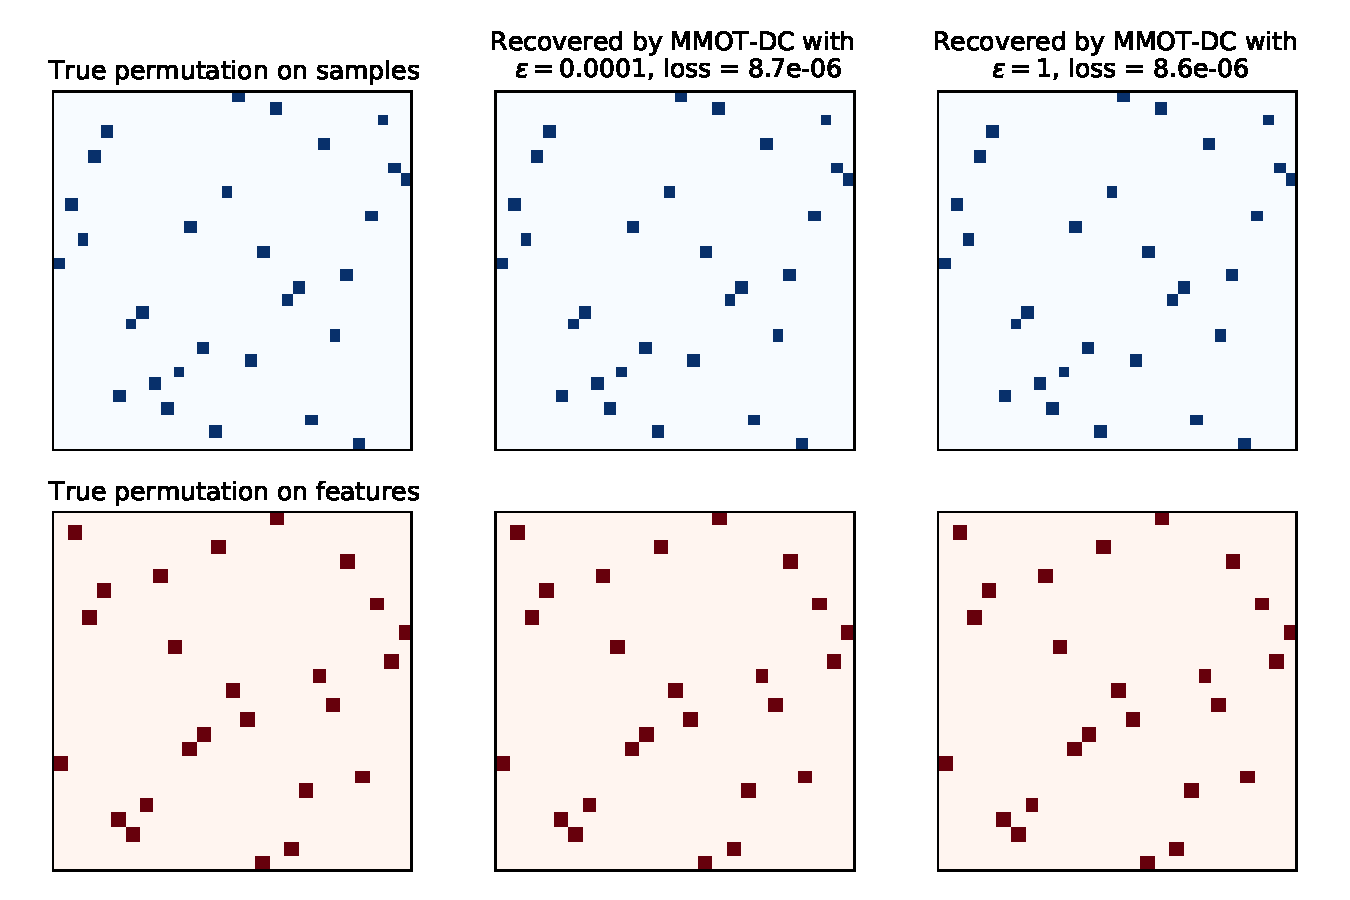
\includegraphics[width=0.8\textwidth,height=0.8\textheight,keepaspectratio]{./Chapitre2/fig/compare_methods.pdf}
  \caption{Couplings generated by COOT and MMOT-DC on the matrix recovering task.}
  \label{fig:permu}
\end{figure}
%%%%%%%%%%%%%%%%%%%%%%%%%%%%%%%%%%%%%%%
We also plot, with some abuse of notation, the histograms of the difference between
the $(1,3), (1,4), (2,3), (2,4)$-marginal matrices of MMOT-DC and their corresponding counterparts from F-MMOT.
In this example, in theory, as the optimal tensor $P$ of F-MMOT can be factorized as
$P = P_{\# \cT_1} \otimes P_{\# \cT_2} = Q_s \otimes Q_f$,
it is immediate to see that $P_{\# (1,3)} = P_{\# (1,4)} = P_{\# (2,3)} = P_{\# (2,4)} \in \bbR^{30 \times 25}$
are uniform matrices whose entries are $\frac{1}{750}$.
%%%%%%%%%%%%%%%%%%%%%%%%%%%%%%%%%%%%%%%
\begin{figure}[t]
  \centering
  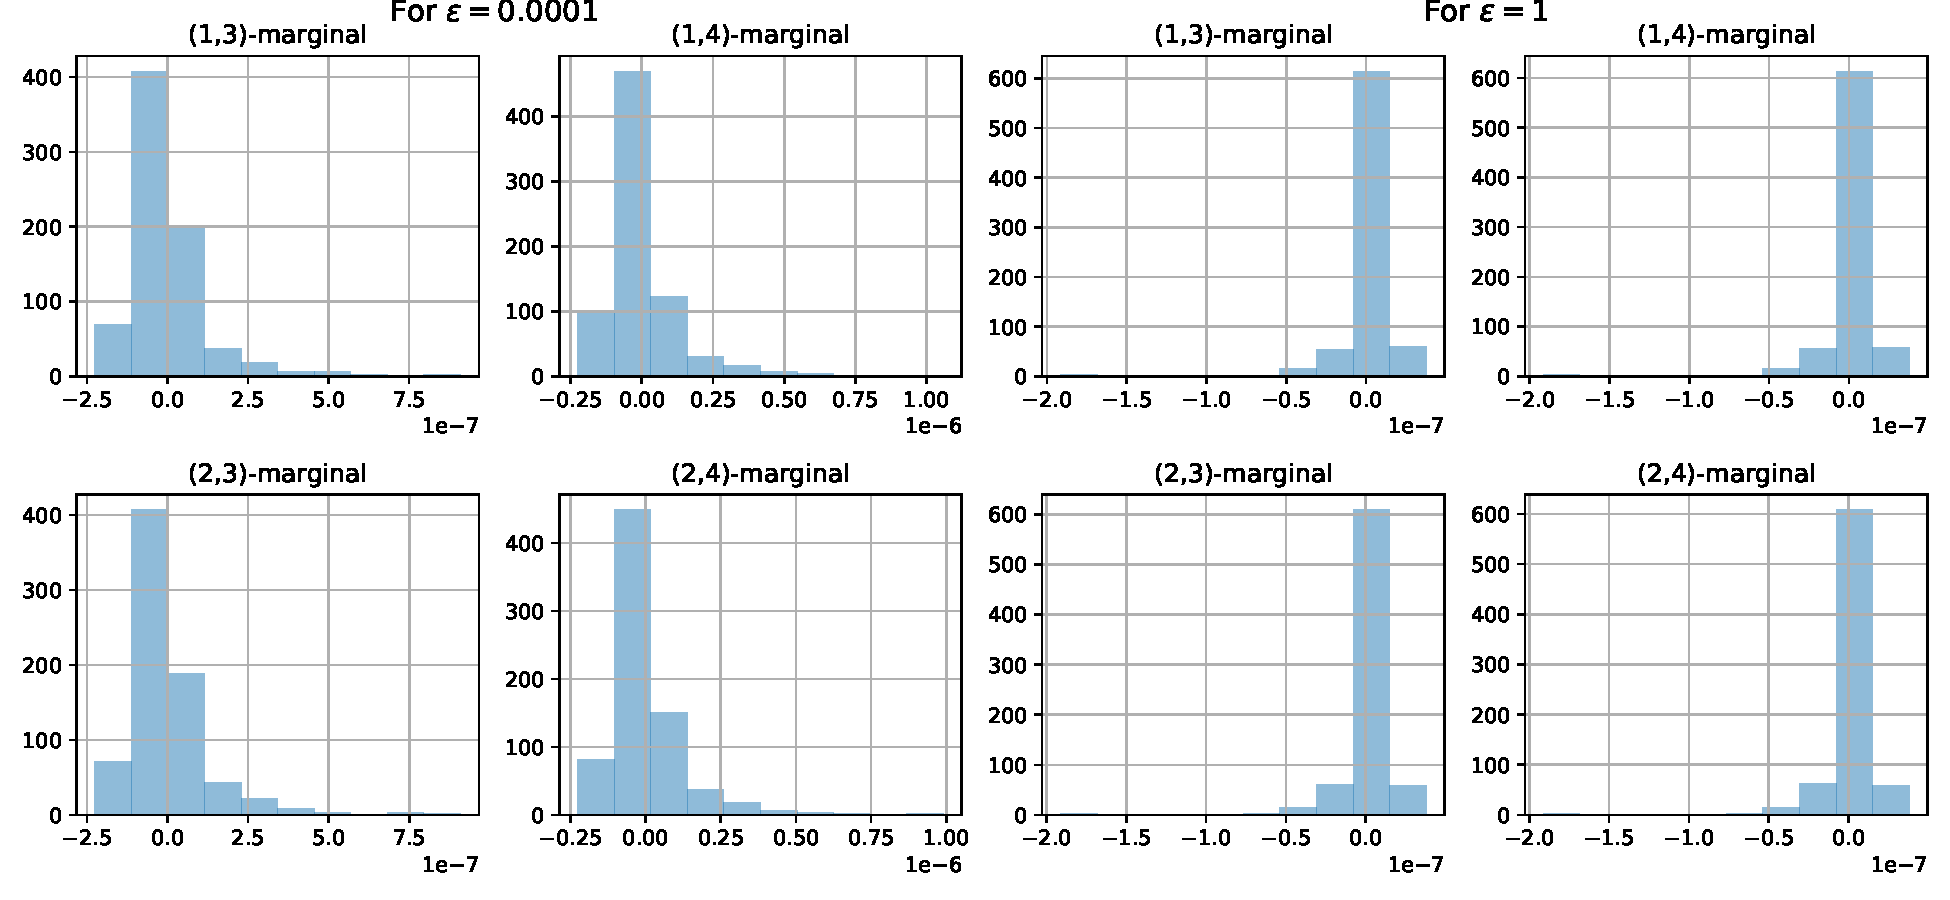
\includegraphics[width=1.\textwidth,height=1.\textheight,keepaspectratio]{./Chapitre2/fig/other_marginals.pdf}
  \caption{Histograms of difference between true independent marginal matrices and their approximations. We see that the marginal matrices obtained
  by \Cref{algo:dc_MMOT} approximate well the theoretical uniform matrices.}
  \label{fig:other_marg}
\end{figure}

%%%%%%%%%%%%%%%%%%%%%%%%%%%%%%%%%%%%%%%
\paragraph{Quality of the MMOT-DC solutions. \label{expe:2}}

% In the following example, our evaluation metric is the COOT loss $\langle C, P \otimes Q \rangle$,
% where the smaller the loss, the better.

Now, we consider the situation where the true matching between two matrices is not known in advance and investigate the quality
of the solutions returned by MMOT-DC to solve the COOT and GW problems. This means that we will look at the COOT loss
$\langle C, Q_s \otimes Q_f \rangle$, where the smaller the loss, the better when using both exact COOT and GW solvers
and our relaxation.

We generate two random matrices $X \in \bbR^{20 \times 3}$ and $Y \in \bbR^{30 \times 2}$,
whose entries are drawn independently from the uniform distribution on the interval $[0,1)$. Then we calculate two corresponding
squared Euclidean distance matrices of size $20$ and $30$. Their rows and columns are equipped with the discrete
uniform distributions. In this case, \citep{Redko20} show that the COOT loss coincides with the GW distance, and the
Block Coordinate Descent (BCD) algorithm used to approximate COOT is equivalent to the Frank-Wolfe algorithm \citep{Frank56}
used to solve the GW distance.

We compare four solvers:
\begin{enumerate}
  \item The Frank-Wolfe algorithm to solve the GW distance (GW-FW).

  \item The projected gradient algorithm to solve the entropic GW distance \citep{Peyre16} (EGW-PGD).
  We choose the regularization parameter from the set
  $\{0.0008, 0.0016, 0.0032, 0.0064, 0.0128, 0.0256 \}$
  and pick the one which corresponds to smallest COOT loss.

  \item The Block Coordinate Descent algorithm to approximate the entropic COOT \citep{Redko20}
  (EGW-BCD), where two additional KL divergences corresponding to two couplings are introduced.

  The regularization parameters are tuned from the set
  $\{0, 0.0005, 0.001, 0.005, 0.01, 0.05, 0.1, 0.5, 1 \}$,
  where $0$ means that there is no regularization term for the corresponding coupling
  and we pick the pair corresponding to the smallest COOT loss.

  \item \Cref{algo:dc_MMOT} to solve the MMOT-DC. We tune
  $\varepsilon \in \{1, 1.4, 1.8, 2.2, 2.6\}$ and we pick the one which corresponds to smallest COOT loss.
\end{enumerate}
For GW-FW and EGW-PGD, we use the implementation from the library \texttt{PythonOT} \citep{Flamary21}.

Given two random matrices, we record the COOT loss corresponding to the solution generated by each method.
We simulate this process $70$ times and compare their overall performance. We can see in \Cref{tab:gw} the average value and
standard deviation and the comparison for the values of the loss between the different algorithms in \Cref{fig:gw}.
The performance is quite similar across methods with a  slight advantage for EGW-PGD. This is in itself a very
interesting result that has never been noted, to the best of our knowledge: the reason that the entropic version of GW can
provide better solution than solving the exact problem, may be due to the "convexification" of the problem, thanks to the entropic
regularization. Our approach is also interestingly better than the exact GW-FW, which illustrates that the relaxation might help in
finding better solutions despite the non-convexity of the problem.
%%%%%%%%%%%%%%%%%%%%%%%%%%%%%%%%%%%%%%%
\begin{table}[t]
  % \vskip 0.15in
  \begin{center}
    \begin{small}
      \begin{sc}
        \begin{tabular}{|c|c|c|c|}
          \hline
          GW-FW & EGW-PGD & EGW-BCD & MMOT-DC \\
          \hline
          0.0829 ($\pm$ 0.0354) & \textbf{0.0786 ($\pm$ 0.0347)} & 0.0804 ($\pm$ 0.0353) & 0.0822 ($\pm$ 0.0364) \\
          \hline
        \end{tabular}
      \end{sc}
    \end{small}
  \end{center}
  \caption{Average and standard deviation of COOT loss of the solvers. MMOT-DC is competitive to other solvers,
  except for EGW-PGD and EGW-BCD.
  \label{tab:gw}}
\end{table}

%%%%%%%%%%%%%%%%%%%%%%%%%%%%%%%%%%%%%%%
\begin{figure}[t]
	\centering
	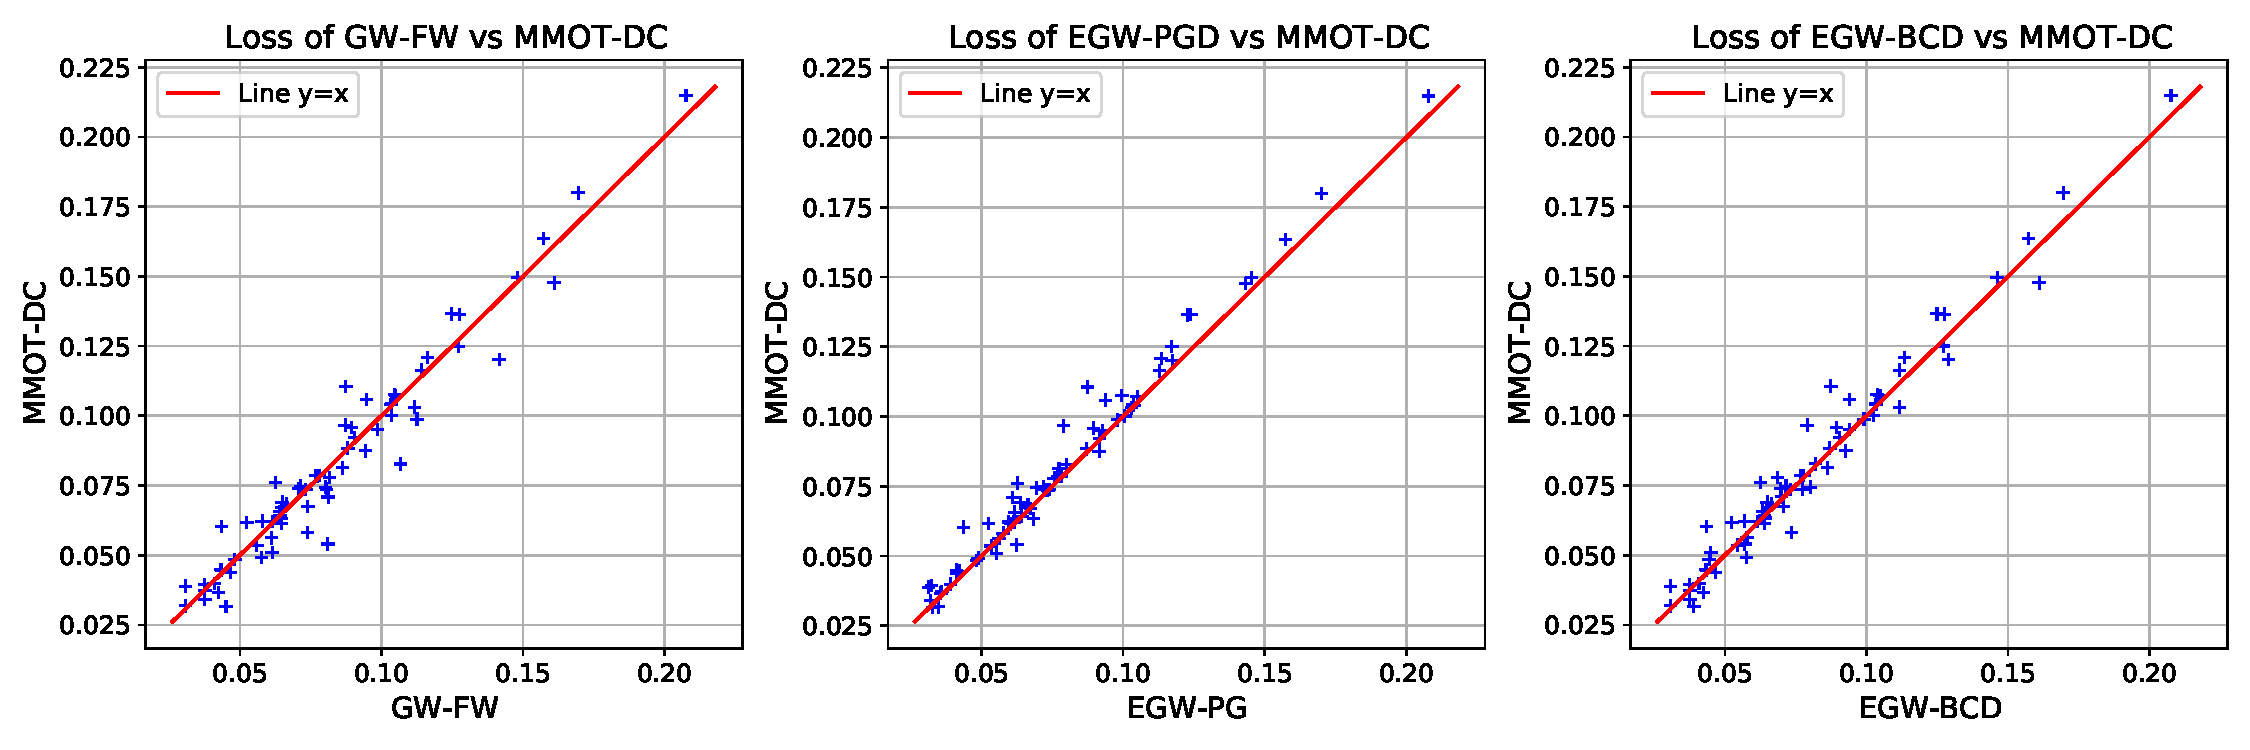
\includegraphics[width=\textwidth,height=\textheight,keepaspectratio]{./Chapitre2/fig/all_vs_MMOT-DC.pdf}
	\caption{Scatter plots of MMOT-DC versus other solvers. In all three plots, the points tend to concentrate around the line $y=x$,
  which indicates the comparable performance of MMOT-DC. On the other hand, the top-right plot shows the clear superiority of EGW-PGD.}
	\label{fig:gw}
\end{figure}
%%%%%%%%%%%%%%%%%%%%%%%%%%%%%%%%%%%%%%%

\paragraph{An empirical variation.} Intuitively, for sufficiently large $\varepsilon$, the minimisation of the KL divergence is prioritised
over the linear term in the objective function of the MMOT-DC problem, which implies that the optimal tensor $P^*$ is "close" to its
corresponding tensor product $P^*_{\# \cT}$. So, instead of calculating the gradient at $P$, one may calculate at
$P_{\# \cT}$. In this case, the gradient reads
\begin{equation}
  \begin{split}
    \sum_{m=1}^M \nabla_P \kl_m(P_{\# \cT}) =
    \log \frac{P_{\# \cT_1}}{\mu^{\otimes}_{\cT_1}} \oplus ... \oplus \log \frac{P_{\# \cT_m}}{\mu^{\otimes}_{\cT_m}} ,
  \end{split}
\end{equation}
where $\oplus$ represents the tensor sum operator between two arbitrary-size tensors: $(A \oplus B)_{i,j}:= A_i + B_j$, where with some
abuse of notation, $i$ or $j$ can be understood as a tuple of indices. Thus, we avoid storing the $N$-D gradient tensor (as in the
\Cref{algo:dc_MMOT}) and only need to store $M$ smaller-size tensors. Not only saving the memory,
this variation also seems to be empirically competitive with the original \Cref{algo:dc_MMOT}, if not sometimes better,
in terms of COOT loss. The underlying reason might be related to the approximate DCA scheme \citep{Thanh15}, where one replaces both
steps in each DC iteration by their approximation. We leave the formal theoretical justification of this variation to the future work.
We call this variation \textit{MMOT-DC-v1} and use the same setup as in Experiment \ref{expe:2}.
\begin{figure}[ht]
  \centering
  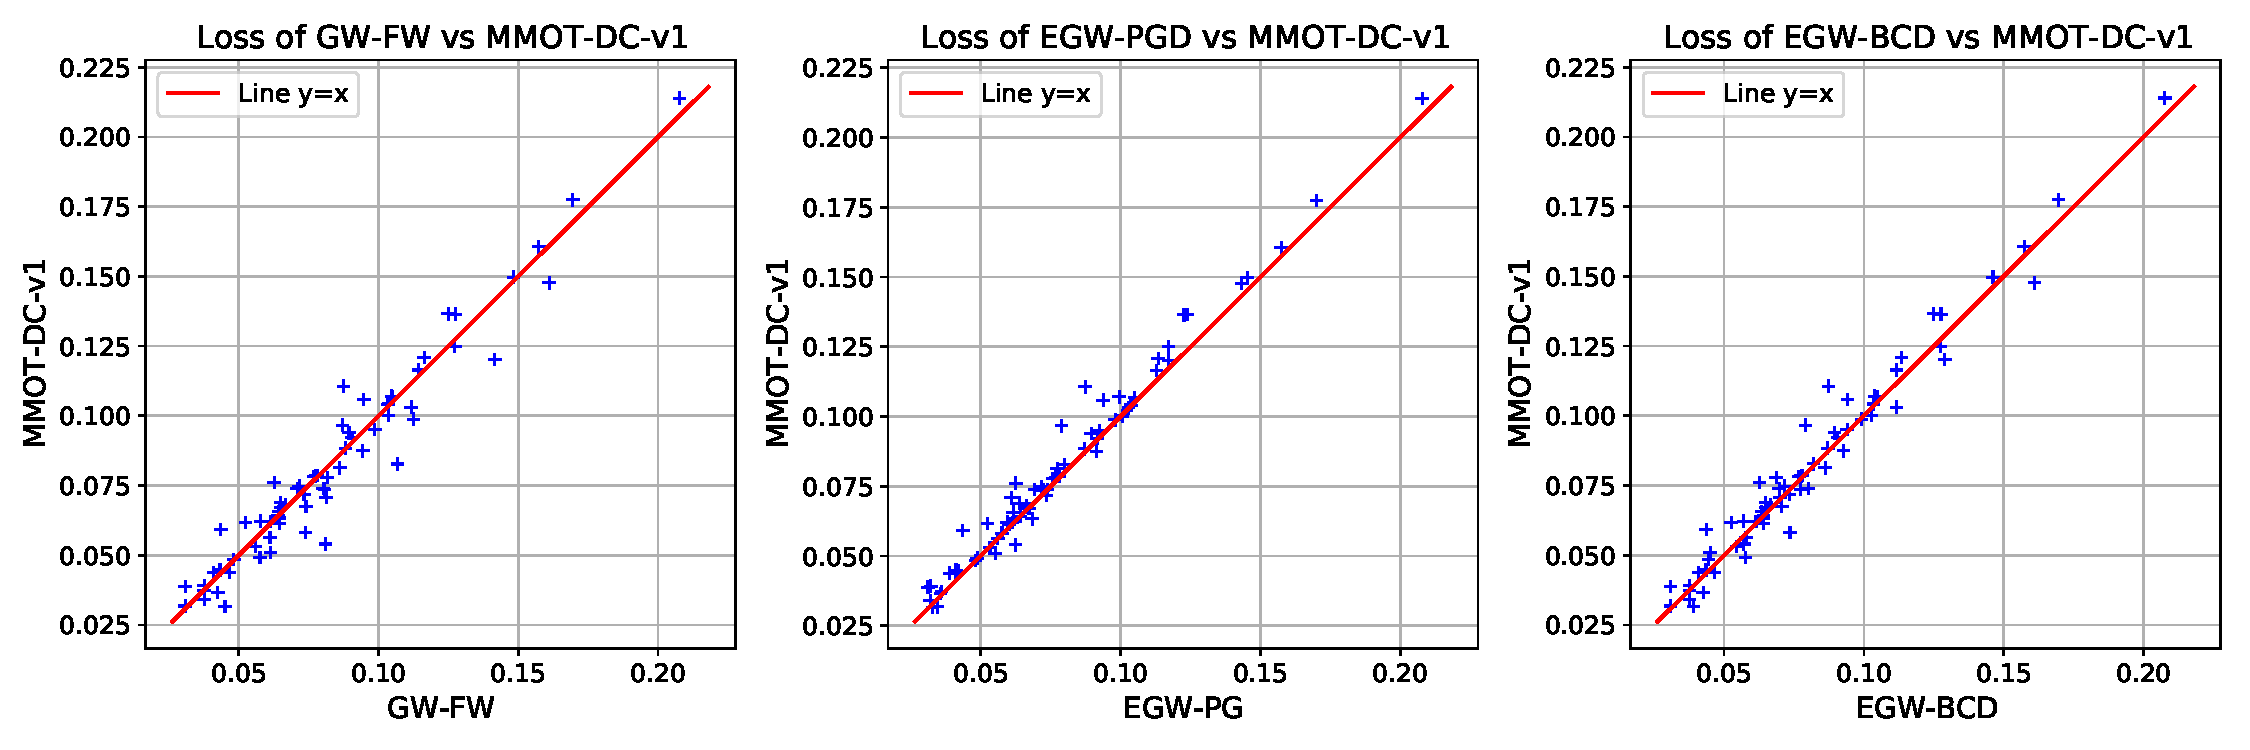
\includegraphics[width=\textwidth,height=\textheight,keepaspectratio]{./Chapitre2/fig/all_vs_MMOT-DC-v1.pdf}
  \caption{Scatter plots of MMOT-DC-v1 versus other solvers. In all three plots, the points tend to concentrate around the line $y=x$,
  which indicates the comparable performance of MMOT-DC-v1. On the other hand, the top-right plot shows the clear superiority of EGW-PGD.}
  \label{fig:coot_mmot_new}
\end{figure}

\begin{table}[H]
  \label{tab:coot_new}
  % \vskip 0.15in
  \begin{center}
    \begin{small}
      \begin{sc}
        \begin{tabular}{|c|c|}
          \hline
          MMOT-DC & MMOT-DC-v1 \\
          \hline
          0.0822 ($\pm$ 0.0364) & 0.0820 ($\pm$ 0.0361) \\
          \hline
        \end{tabular}
      \end{sc}
    \end{small}
  \end{center}
  \caption{Average and standard deviation of COOT loss of MMOT-DC and MMOT-DC-v1. The performance of the two algorithms is
  very similar.}
  % \vskip -0.1in
\end{table}

%%%%%%%%%%%%%%%%%%%%%%%%%%%%%%%%%%%%%%
\subsection{Conclusion and future work}
%%%%%%%%%%%%%%%%%%%%%%%%%%%%%%%%%%%%%%

In this paper, we present a novel relaxation of the factorized MMOT problem called \textit{MMOT-DC}.
More precisely, we replace the
hard constraint on factorization constraint by a smooth regularization term. The resulting problem
not only enjoys an interpolation property between MMOT and factorized MMOT, but also is a DC problem,
which can be solved easily by the DC algorithm. We illustrate the use of MMOT-DC the via some simulated experiments and show that
it is competitive with the existing popular solvers of COOT and GW distance.
One limitation of the current DC algorithm is that, it is not scalable because
it requires storing a full-size tensor in the gradient step computation. Thus, future
work may focus on more efficiently designed algorithms, in terms of both time and memory footprint.
Moreover, incorporating additional structure on the cost tensor may also be computationally and practically beneficial.

From a theoretical viewpoint, one potential application of MMOT-DC is on the study of the sample complexity of GW distance.
More precisely, given two measure networks $\cX = (X, c_X, \mu_X)$ and $\cY = (Y, c_Y, \mu_Y)$,
we want to quantify $| \gw(\cX, \cY) - \gw(\cX_n, \cY_n)|$. Note that, \citep{Zhang23} has also
established the convergence rate for the case of $2$-GW distance, in which the cost function
is the squared Euclidean distance. Our proposed approach, if works, would be able to handle any
conditionally negative (or positive) semi-definite kernel.

The idea is as follows: by \Cref{prop:coot_gw_equiv}, COOT and GW distance are equivalent
\footnote{Note that one needs to properly extend \Cref{prop:coot_gw_equiv} to the continuous setting
(of measure networks).}. So, we can replace GW by COOT, as it is less (unnecessarily) constrained.
Next, we extend MMOT-DC to the continuous setting and show that the interpolation property
still holds, notably MMOT-DC converges to COOT as regularization tends to the infinity.
Thanks to the DC algo, we can linearize the MMOT-DC and obtain an entropic MMOT problem.
This problem has two advantages. First, one can reuse the technique for entropic OT
in \citep{Genevay19} and extend to the entropic MMOT. Second, for suitable choice of input,
it approximates COOT.

Note that, this is still an ongoing work as we have not yet fully resolved all
technical difficulties. Nevertheless, we report the sketch of the proof and leave most of
mathematical details in Appendix.

\paragraph{Assumptions} We assume that the measure networks
$\cX = (X, c_X, \mu_X)$ and $\cY = (Y, c_Y, \mu_Y)$. $X$ and $Y$ are compact
subsets of $\bbR^{d_x}$ and $\bbR^{d_y}$, respectively. The probability measures
$\mu_X$ and $\mu_Y$ are absolutely continuous with respect to the Lebesgue measures
on $\bbR^{d_x}$ and $\bbR^{d_y}$, respectively.
With some abuse of notation, we also use $\mu_X, \mu_Y$ to denote their density functions.

\paragraph{Sketch of proof}
For convenience, denote $\cU_4 = U(\mu_X, \mu_Y, \mu_X, \mu_Y)$ and $\mu = \mu_X \otimes \mu_Y$.
We write $c = |c_X - c_Y|^2$ defined by $c(x, y, x', y') = |c_X(x, x') - c_Y(y, y') |^2$.
Recall that, for any $\pi \in \cU_4$, we denote $\pi_{\#} = \pi_{\# 12} \otimes \pi_{\# 34}$.
\begin{lemma}
  For each $\pi \in \cU_4$, denote
  $G(\pi) := \kl(\pi_{\# 12} | \mu) + \kl(\pi_{\# 34} | \mu) = \kl(\pi_{\#} | \mu^{\otimes 2})$.
  Then $G$ is convex and differentiable. In particular, $G(\pi) = \int \nabla G(\pi) \; d \pi$,
  for $\pi \in \cU_4$.
\end{lemma}
Now, we have
\begin{align}
  \int c \; d\gamma + \varepsilon \kl(\gamma | \gamma_{\#})
  &\leq \int c \; d\gamma + \varepsilon \kl(\gamma | \mu^{\otimes 2})
  - \varepsilon \Big[ G(\pi) + \int \nabla G(\pi) \; d \gamma - \int \nabla G(\pi) \; d \pi \Big] \\
  &= \int \big[ c - \varepsilon \nabla G(\pi) \big] \; d \gamma
  + \varepsilon \kl(\gamma | \mu^{\otimes 2}).
\end{align}
By taking infimum over $\cU_4$, we obtain
\begin{align}
  \mmotdc_{\varepsilon} \leq
  \inf_{\gamma \in \cU_4} \int \big[ c - \varepsilon \nabla G(\pi) \big] d \gamma
  + \varepsilon \kl(\gamma | \mu^{\otimes 2}).
\end{align}
Now, we define the following MMOT problem.
\begin{definition}
  For $\pi \in \cU_4$, define
  \begin{align}
    \mmot_{\varepsilon}\big( c - \varepsilon \nabla G(\pi) \big) :=
    \inf_{\gamma \in \cU_4} \int \big[ c - \varepsilon \nabla G(\pi) \big] \; d \gamma
      + \varepsilon \kl(\gamma | \mu^{\otimes 2}).
  \end{align}
\end{definition}
There exists $\pi \in \cU_4$ such that $\mmot_{\varepsilon}\big( c - \varepsilon \nabla G(\pi) \big)$
approximates COOT. For example, denote $\pi_{\varepsilon}$
the solution of the entropic COOT problem $\coot_{\varepsilon}(\cX, \cY)$, we can show that
\begin{corollary}
  For every $\varepsilon > 0$, we have
  $\coot_{1 / \varepsilon}(\cX, \cY) \geq
  \mmot_{\varepsilon}\big( c - \varepsilon \nabla G(\pi_{1 / \varepsilon}) \big) \geq \mmotdc_{\varepsilon}$.
  As a consequence,
  $\mmot_{\varepsilon}\big( c - \varepsilon \nabla G(\pi_{1 / \varepsilon}) \big) \to \coot(\cX, \cY)$,
  when $\varepsilon \to \infty$.
\end{corollary}
Now, suppose $\mmot_{\varepsilon}\big( c - \varepsilon \nabla G(\pi^*) \big)$ can approximate COOT,
for some $\pi^* \in \cU_4$. Then, by the triangle inequality, we have
\begin{align}
  | \coot_(\cX, \cY) - \coot_(\cX_n, \cY_n)|
  &\leq |\coot_(\cX, \cY) - \mmot_{\varepsilon}\big( c - \varepsilon \nabla G(\pi^*) \big)| \\
  &+ |\mmot_{\varepsilon, n}\big( c - \varepsilon \nabla G(\pi^*) \big) - \mmot_{\varepsilon}\big( c - \varepsilon \nabla G(\pi^*) \big)| \\
  &+ |\coot(\cX_n, \cY_n) - \mmot_{\varepsilon, n}\big( c - \varepsilon \nabla G(\pi^*) \big)|,
\end{align}
Now, it is enough to bound each term and obtain the final rate. However, the main difficulties
lie on finding the appropriate choice of $\pi^*$ and on how to control
it in the entropic MMOT problem.

% \subsection{Stability of Co-Optimal Transport}

% COOT setting: given two sample-feature spaces
% $\cX_1 = ((X_1^s, \mu_1^s), (X_1^f, \mu_1^f), \xi_1)$ and
% $\cX_2 = ((X_2^s, \mu_2^s), (X_2^f, \mu_2^f), \xi_2)$. COOT reads
% \begin{equation}
%     \coot(\cX_1, \cX_2) =
%     \inf_{\substack{\pi^s \in U() \\ \pi^f \in U()}}
%     \int |\xi_1 - \xi_2|^2 d\pi^s d\pi^f
% \end{equation}
% Consider the "semi-empirical" spaces:
% $\widehat{\cX}_i := ((\widehat{X}_i^s, \widehat{\mu}_i^s), (X_i^f, \mu_i^f), \xi_i))$, where
% we fix the dimension $f$ and only consider the empirical version of sample measures.
% Now, how does the feature coupling behave when $\widehat{\mu}^s \to \mu^s$?, i.e. when $n \to \infty$,
% quantify
% \begin{equation}
%     | \coot(\cX_1, \cX_2) -
%     \coot(\widehat{\cX}_1, \widehat{\cX}_2) |
% \end{equation}
% We can first start with finite-dimensional feature spaces (so the feature coupling is a matrix).

\vfill